\section{Healthcare services accessibility}

\subsection{Italian overview}

Accessibility to healthcare services is a key determinant of population well-being and social equity. 
Ensuring that people can reach medical facilities within a reasonable time is essential for timely diagnosis, treatment, and prevention of health conditions. 
Differences in accessibility often reflect broader regional disparities, influencing quality of life, economic opportunities, and demographic sustainability. 
Studying healthcare accessibility therefore provides valuable insights for politician, helping to identify underserved areas and design more inclusive health systems.

Figure \ref{map:acc_by_region_2023n1} show the mean accessibility time to reach the nearest hospital structure for Italian regions, it is expressed as driving minutes to the nearest medical centre.
Classification was realized categorizing mean times in intervals of equal dimension, technique which allows us to highlight regions that have better or worse average times.
As can be seen from the graph, Northern Italy tends to have lighter colours, a sign of easier access to health centres.
The most virtuous region of the peninsula proves to be Lombardia, with an average time of 12 minutes; on the other side of the ranking, Valle d'Aosta and Sardegna show the worst values, with average times up to 26 minutes.

If we look at the map showing the travel time to the three closest healthcare facilities (Figure \ref{map:acc_by_region_2023n3}), the situation changes slightly. 
For some regions, such as Trentino-Alto Adige and Basilicata, the situation worsens, placing them in the lowest class; for other regions, especially in central Italy, the situation improves slightly.


\begin{figure}[tbp]
	\centering
	\includegraphics[width=0.5\textwidth]{img/Accessibilità per regione.pdf}
	\caption{Accessibility to the nearest healthcare service by region in 2023}
	\label{map:acc_by_region_2023n1}
\end{figure}

\begin{figure}[tbp]
	\centering
	\includegraphics[width=0.5\textwidth]{img/Accessibilità per regione n3.pdf}
	\caption{Accessibility to the 3 nearest healthcare services by region in 2023}
	\label{map:acc_by_region_2023n3}
\end{figure}


When reading these maps, one must not forget the nature of the Italian territory, which is mountainous in many areas.
While urban and lowland areas often benefit from dense networks of medical facilities and efficient transport connections, many mountainous and rural regions face significant challenges. 
Steep terrain, dispersed settlements, and limited infrastructure can increase travel times to healthcare centres, creating disparities in access to essential services. 


\subsection{North of Italy}

Let us now turn to northern Italy, a region chosen for its wide range of environments: an extensive plain, mountain ranges, and coastal areas.
Access times have been organised into 4 categories:
\begin{center}
\begin{tabular}{l c l}
	\toprule
	\textbf{No.} & \textbf{Travel time} & \textbf{Accessibility}\\
	& [min] & \\
	\midrule
	1 & < 15 & High\\
	2 & [15, 30) & Medium-high\\
	3 & [30, 45) & Medium-low\\
	4 & > 45 & Low\\
	\bottomrule
\end{tabular}
\end{center}
\medskip

From Figure \ref{map:acc_by_comm_classes_2023n1} we note that Pianura Padana benefit of an excellent coverage in terms of health facilities, indeed it is the most populous and productive area in Italy, where there are no natural obstacles hampering connections or construction of new facilities.

This situation stays almost the same when considering accessibility to the three closest structures (Figure \ref{map:acc_by_comm_classes_2023n3}).
The most densely populated areas do not experience any changes in category when considering the closest centre or the first three. 
This is the case of the provinces of Milan, Como, Bergamo, and the areas along A1 highway. 
People living in the aforementioned areas can reach a great number of medical centres driving less than 15 minutes.

The situation changes considerably when we look at the outer reaches of northern Italy, near the border, where the Italian territory is crossed by the Alpine mountain range, a natural border with neighbouring France, Switzerland, Austria, and Slovenia.
The morphology of these areas, coupled with their lower population density and a less efficient road infrastructure, makes them much less accessible from a healthcare perspective.
In mountainous areas near the border, travel times often exceed 15 minutes to the nearest healthcare facility, and consistently exceed 30 minutes to reach the three closest facilities.


\begin{figure}[tbp]
	\centering
	\includegraphics[width=\textwidth]{img/Accessibilità per comune in 4 classi N.pdf}
	\caption{Accessibility by class to reach the closest healthcare service in 2023}
	\label{map:acc_by_comm_classes_2023n1}
\end{figure}

\begin{figure}[tbp]
	\centering
	\includegraphics[width=\textwidth]{img/Accessibilità per comune in 4 classi N 2023n3.pdf}
	\caption{Accessibility by class to reach the 3 closest healthcare services in 2023}
	\label{map:acc_by_comm_classes_2023n3}
\end{figure}

As shown in the histogram in Figure \ref{hist:acc_by_class_N_2023n1}, Northern Italy displays a favorable distribution of healthcare facilities, with 60\% of municipalities located within a 15-minute drive of a facility and 92\% within 30 minutes.

\begin{figure}[tbp]
	\centering
	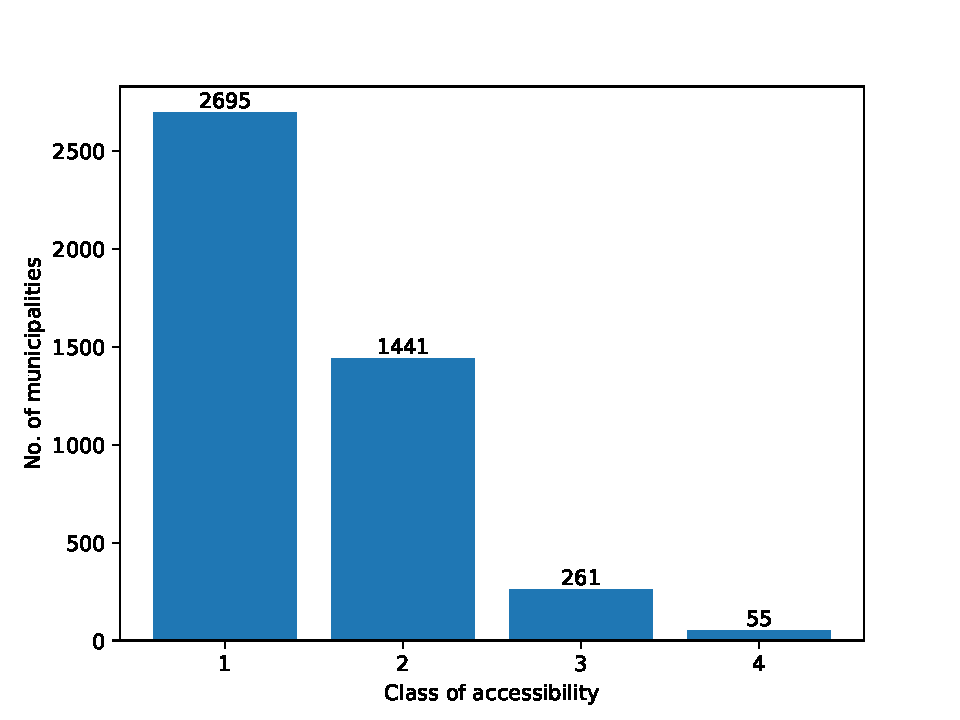
\includegraphics[width=0.7\textwidth]{img/acc_comm_by_class_North_2023n1.pdf}
	\caption{Distribution of accessibility classes in Northern Italy municipalities. Time to reach the closest healthcare service in 2023}
	\label{hist:acc_by_class_N_2023n1}
\end{figure}


\subsection{Population living in areas with poor healthcare accessibility}

We can calculate the portion of population living in the municipalities of each class, results are shown in the following table.

\smallskip
\begin{center}
\begin{tabular}{r S[table-format=8.0] S[table-alignment-mode=marker]}
	\toprule
	\textbf{Class} & \textbf{Population} & \textbf{\% of total}\\
	\midrule
	1 & 18836153 & 69.32\\
	2 & 7399725 & 27.23\\
	3 & 792058 & 2.91\\
	4 & 143979 & 0.53\\
	  & 27171915 & \\
	\bottomrule
\end{tabular}
\end{center}
\smallskip

Based on time needed to reach the 3 closest health facilities, we consider those in classes 3 and 4 as municipalities with poor health accessibility.
There are 936037 people living in communes of the two lower classes, equivalent to 3.44\% of the population.

Overall, the distribution of the population across classes shows a generally favourable situation, with more than 96\% of residents living in municipalities classified as 1 or 2, where access to healthcare facilities is relatively fast.
Nevertheless, almost one million people (3.44\% of the total population) live in municipalities belonging to classes 3 and 4, which indicates limited accessibility to healthcare services. 
As discussed before, these areas coincide with sparsely populated rural or mountain regions, where lower population density and geographical barriers constrain the availability of facilities.


\begin{figure}[tbp]
	\centering
	\begin{subfigure}{\textwidth}
		\centering
		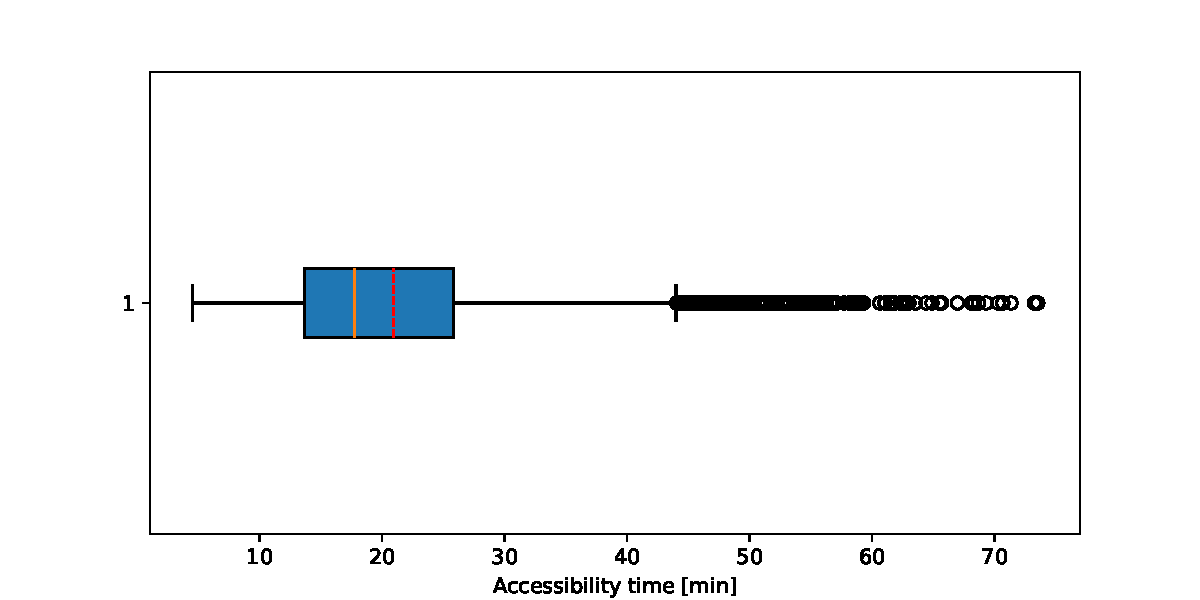
\includegraphics[width=0.8\linewidth]{img/boxplot_acc_by_comm_2023n3.pdf}
		\caption{Boxplot of accessibility times}
		\label{boxplot:acc_by_comm_2023n3}
	\end{subfigure}
	\medskip
	
	\begin{subfigure}{\textwidth}
		\centering
		\begin{tabular}{l S[table-alignment-mode=marker]}
			\toprule
			\textbf{Index} & \textbf{Value}\\
			\midrule
			Q1 (25\%) & 13.66\\
			Median (50\%) & 17.75\\
			Q3 (75\%) & 25.8\\
			Mean & 20.92\\
			IQR & 12.14\\
			\bottomrule
		\end{tabular}
		\caption{Boxplot statistics for accessibility times}
		\label{tab:boxplot_idxs}
	\end{subfigure}
	
	\caption{Distribution of municipal accessibility times to the three closest healthcare facilities}
\end{figure}


\subsection{Change in healthcare accessibility between 2020 and 2023}

This section analyses the change in accessibility to reach the nearest healthcare facility between 2020 and 2023.
The 7 intervals of change reported in Table \ref{tab:acc_variation_classes} have been defined.

\begin{table}[tb]
	\centering
\begin{tabular}{l c S[table-format=4.0]}
	\toprule
	\textbf{Class} & \textbf{Interval} [\%] & \textbf{No. communes}\\
	\midrule
	Sharp worsening & $\linterval{-\infty}{20}$ & 135\\
	Relevant worsening & $\linterval{-20}{-10}$ & 348\\
	Slight worsening & $\linterval{-10}{-5}$ & 586\\
	No change & $\interval[open]{-5}{5}$ & 2298\\
	Slight improvement & $\rinterval{5}{10}$ & 494\\
	Relevant improvement & $\rinterval{10}{20}$ & 355\\
	Sharp improvement & $\rinterval{20}{+\infty}$ & 236\\
	\bottomrule
\end{tabular}
	\caption{Number of municipalities in each class of percentage change in access time to the nearest health centre}
	\label{tab:acc_variation_classes}
\end{table}

\begin{figure}[tbp]
	\centering
	\includegraphics[width=\textwidth]{img/var accessibilità n1 nord.pdf}
	\caption{Percentage variation of accessibility times to reach the closest medical centre from 2020 to 2023 by commune}
	\label{map:acc_variation_n1}
\end{figure}

As can be seen from Figure \ref{map:acc_variation_n1}, the majority of municipalities have not undergone significant changes in access times to medical facilities.
Percentage change in time was obtained with the following query, using this formula:
\begin{equation*}
	\Delta_{n3} [\%] = \frac{\overline{t}_{2023n1} - \overline{t}_{2020n1}}{\overline{t}_{2020n1}} * 100
\end{equation*}

\begin{minted}{sql}
SELECT 
	c."COMM_ID",
	c."COMM_NAME",
	c.mean_health_2020_n1,
	c.mean_health_2023_n1,
	ROUND(((c.mean_health_2023_n1 - c.mean_health_2020_n1) / c.mean_health_2020_n1 * 100.0)::NUMERIC, 2) as variation_n1,
	c.geom
FROM it_communes c
WHERE SUBSTRING(c."NUTS_CODE" FROM 1 FOR 3) IN ('ITC','ITH');
\end{minted}


We report here the count of the municipalities that fall into each class in Table \ref{tab:acc_variation_classes}.




















